\documentclass[a4paper,11pt]{article}
\setlength{\topmargin}{-.5in}
\setlength{\textheight}{9in}
\setlength{\oddsidemargin}{.125in}
\setlength{\textwidth}{6.25in}
\usepackage[pdftex]{graphicx}
\makeatletter
\renewcommand\paragraph{%
   \@startsection{paragraph}{4}{0mm}%
      {-\baselineskip}%
      {.5\baselineskip}%
      {\normalfont\normalsize\bfseries}}
\makeatother

\begin{document}

% The Title page
\begin{titlepage}
\begin{center}

\includegraphics[width=0.8\textwidth]{fig/eorlogo}\\[3cm]    
\textsc{\LARGE LEDDB description and usage}\\[0.5cm]
\vfill
{\large 
\emph{Oscar Martinez} \\
University of Groningen \\ 
Kapteyn Astronomical Institute \\
Groningen \\
The Netherlands \\
\today}
\end{center}
\end{titlepage}

% INDEX
\tableofcontents
\newpage


\section {Introduction}

This document describes the \textbf{L}OFAR \textbf{E}oR \textbf{D}iagnostic \textbf{D}ata\textbf{B}ase (LEDDB): its ``raison d'etre", contents, implementation, updating, maintenance, etc. 

It also describes the LEDDB web UI focusing on the type of queries the user can make and how to optimally configure them. 

There is also a brief chapter about how to use the query results to do some LOFAR EoR data management and processing as well as diagnostic data analysis. 

If you are only interested in an example of usage, go to section~\ref{sec:usageexample}.

\section {LEDDB overview}

The goal of the LOFAR EoR group is to study the redshifted 21-cm line of neutral hydrogen from the Epoch of Reionization. To meet this goal it requires hundreds of hours of observation thereby accumulating petabytes of data. To diagnose and monitor the various instrumental and ionospheric parameters, as well as manage the data, we have developed the LEDDB. Hence, its tasks are:

\begin{itemize}
	\item To store referencing information of the LOFAR EoR observations, mainly the locations of the data but also other indexing information.
	
	\item To store diagnostic parameters, related to the instrument and ionosphere, extracted through the calibration of these observations. Currently the complex gain solutions and the quality statistics are stored. 
\end{itemize}

Its uses are:
\begin{itemize}
	\item To facilitate efficient data management and pipeline processing.
	
	\item To monitor the performance of the telescope as a function of date.
	
	\item To visualize the diagnostic parameters. This includes tools for the generation of plots and animations to analyze the diagnostic data through all its multiple dimensions. For example we can observe the complex gain of all the stations as a function of time and frequency to visualize ionospheric distortion affecting large part of the array.
\end{itemize}

\subsection{Content}

The content of the database is categorized under three different blocks: the referencing information, the diagnostic data and the meta-data. 

In the referencing information and diagnostic data blocks there are two types of tables: the primary tables and the secondary tables. The primary tables are the core of the LEDDB, i.e. the ones containing the data. The secondary tables add consistency and normalization to the database. They also ease the filtering of the primary tables because we can see the different values that certain column in a primary table can have.

In figure \ref{fig:leddber} we show the Entity-Relationship diagram of the database with its blocks, the tables involved and their relationships. 

\begin{figure}[h]
	\centering
	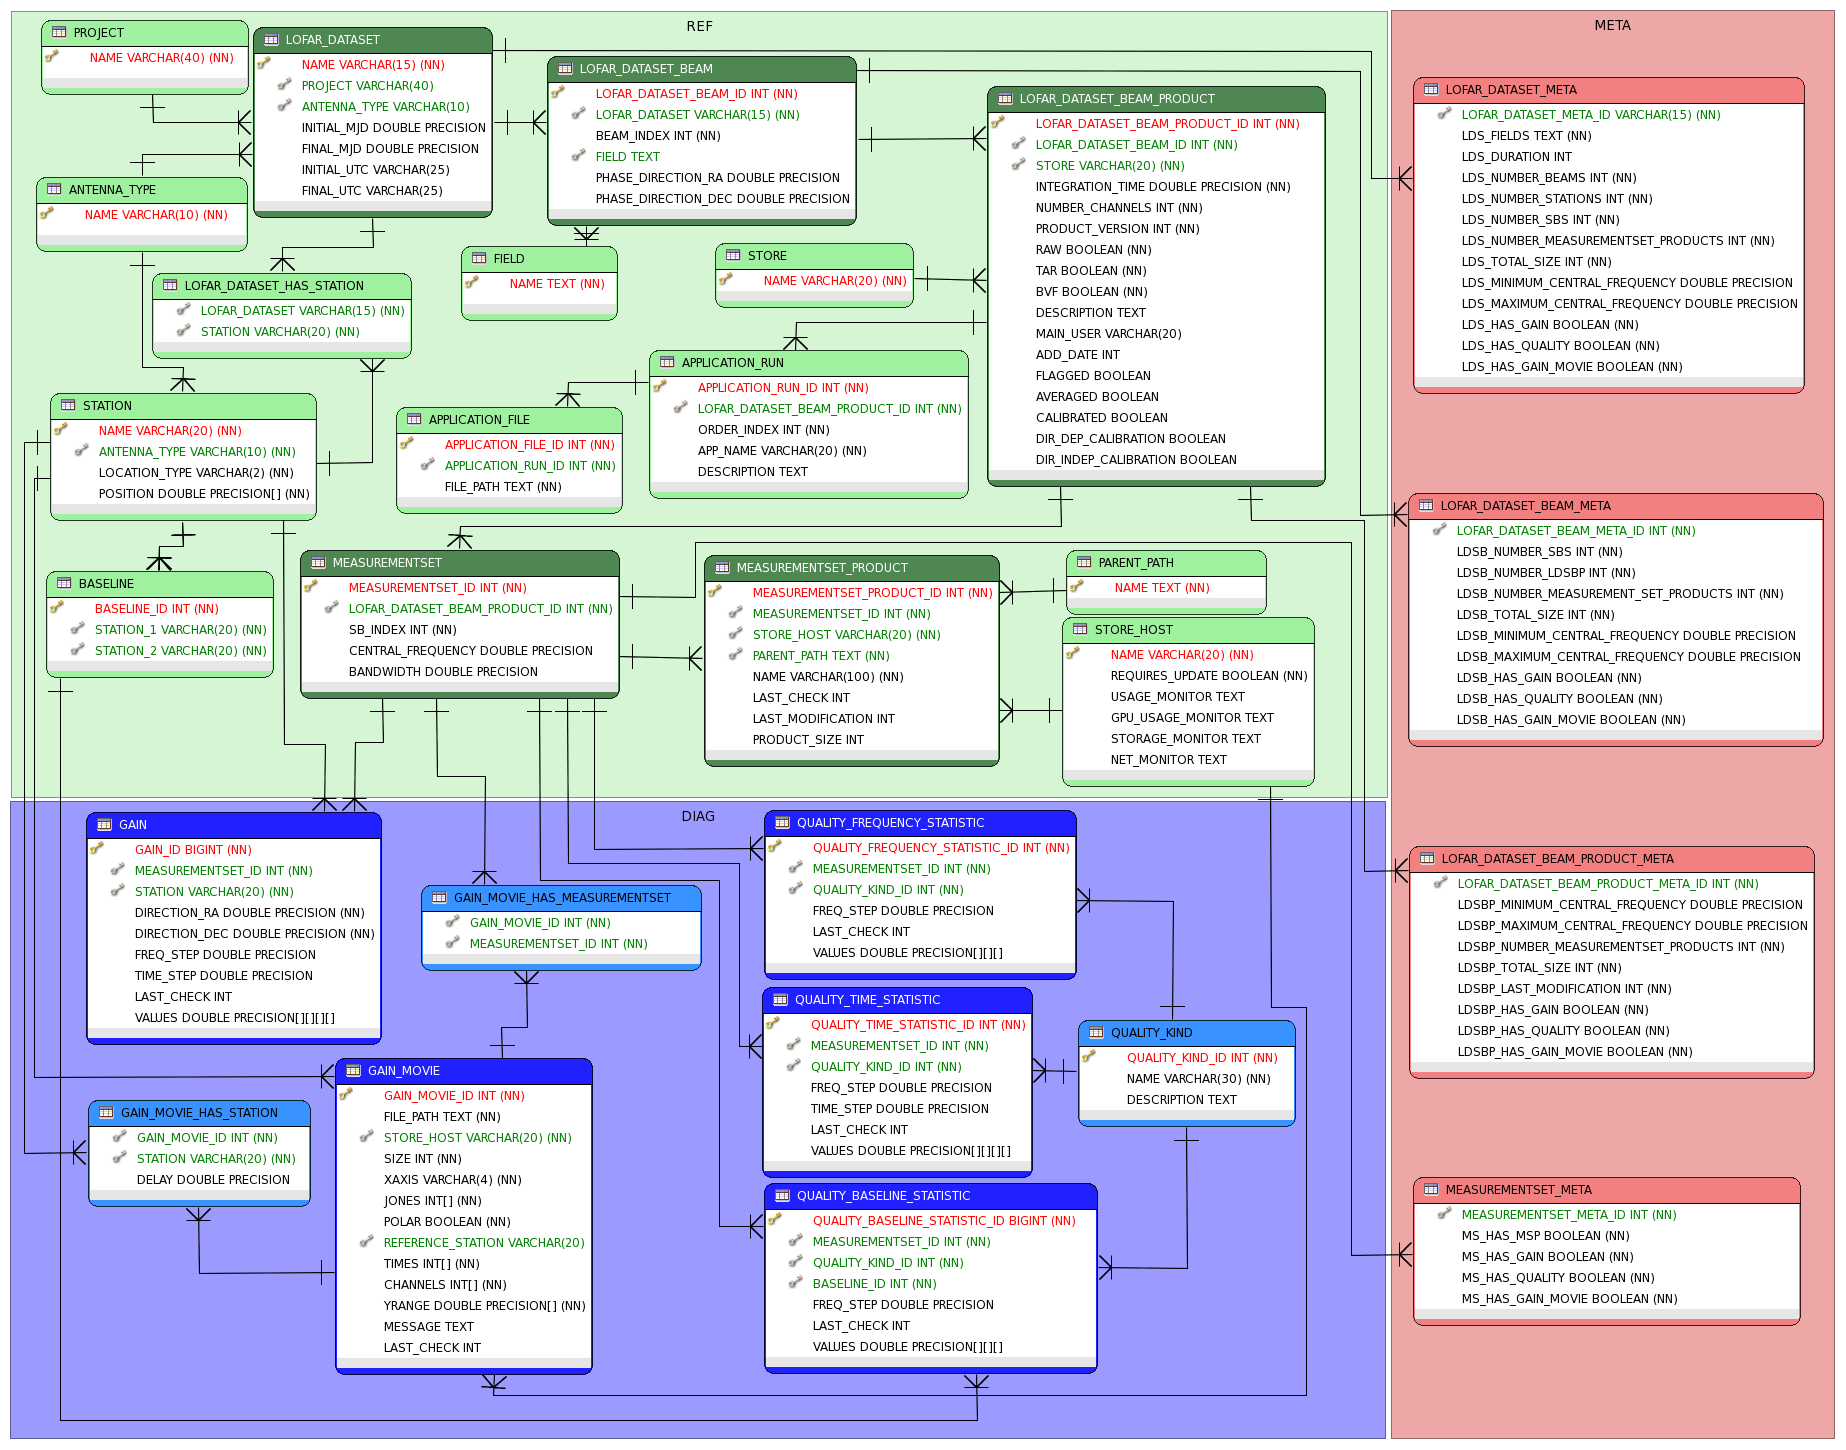
\includegraphics[scale=0.25]{fig/leddber} 
	\caption{Entity-Relationship Diagram of the LEDDB}
	\label{fig:leddber}
\end{figure}

\subsubsection{Referencing information}
\label{sec:ref}

The Referencing information block (\textit{``REF''} in figure \ref{fig:leddber}) contains information for the proper indexing of the different observations done by the LOFAR EoR group, as well as the locations (the cluster and host the data is in and the path to the files) of the data related to such observations. It contains the following primary tables:

\begin{itemize}
	\item \textit{LOFAR\_DATASET} (LDS): This refers to information of an observation done by LOFAR. This includes name of the observation, the project it belongs to, date and time information and the type of antennas that were used.
	
	\item \textit{LOFAR\_DATASET\_BEAM} (LDSB): For multiple beams observations we will have a different entry for each beam in this table. Here we can find the pointed field of each beam.
	
	\item \textit{LOFAR\_DATASET\_BEAM\_PRODUCT} (LDSBP): This refers to some actual data related to an entry in the LDSB table. For the same LDSB entry we can have different LDSBP depending on where the data is stored (LOFAR EoR cluster, TARGET LTA, etc...), the packing type (TAR, BVF or none) and the averaging properties in frequency and time.
	
	\item \textit{MEASUREMENTSET} (MS): This refers to frequency information (sub-band index, central frequency and bandwidth) of each one of the measurement sets of a LDSBP.
	
	\item \textit{MEASUREMENTSET\_PRODUCT} (MSP): This is the location of data related to a measurement set, which must be related to an entry in the table MS. The difference between MS and MSP is that if we delete (or archive elsewhere) the measurement set data, the entry in the MSP table should be deleted but not the one in MS (we still want to know that at some point that measurement set existed). 
\end{itemize}

There also some secondary tables: PROJECT, ANTENNA\_TYPE, FIELD, STATION (and LOFAR\_DATASET\_HAS\_STATION), STORE, BASELINE, STORE\_HOST and PARENT\_PATH.

In this block there are also the tables APPLICATION\_RUN and APPLICATTION\_FILE. These tables are used to describe the processing steps that have been performed over a LDSBP. They are used to generate SIPs (XML meta-data required for TARGET LTA).

\subsubsection{Diagnostic data}
\label{sec:diag}

The diagnostic data block (\textit{``DIAG''} in figure \ref{fig:leddber}) contains the diagnostic parameters related to the observations. The are five primary tables:

\begin{itemize}
	\item \textit{QUALITY\_BASELINE\_STATISTIC} (QBS): Baseline-based statistical parameters extracted and reformatted from the quality statistic sub-table \textit{QUALITY\_BASELINE\_STATISTIC} of each measurement set. A row contains quality baseline statistic for a certain MS, baseline and quality kind. The values are stored as a three dimensional matrix. The dimensions are polarization cross-correlation, frequency channel and complex coordinate. 
	
	\item \textit{QUALITY\_FREQUENCY\_STATISTIC} (QFS): Frequency-based statistical parameters extracted and reformatted from the quality statistic sub-table \textit{QUALITY\_FREQUENCY\_STATISTIC} of each measurement set. A row contains quality frequency statistic for a certain MS and quality kind. The values are stored as a three dimensional matrix. The dimensions are polarization cross-correlation, frequency channel and complex coordinate. 
	
	\item \textit{QUALITY\_TIME\_STATISTIC} (QTS): Time-based statistical parameters extracted and reformatted from the quality statistic sub-table \textit{QUALITY\_TIME\_STATISTIC} of each measurement set. A row contains quality time statistic for a certain MS and quality kind. The values are stored as a four dimensional matrix. The dimensions are polarization cross-correlation, frequency channel, time and complex coordinate. 
	
	\item \textit{GAIN}: This table contains complex gain solutions of the stations (currently only from BBS, later also SAGECAL derived solutions). A row contains the gain solutions for certain MS, station and direction. The values are stored as a four dimensional matrix. The dimensions are polarization cross-correlation, frequency channel, time and complex coordinate. 
	
	\item \textit{GAIN\_MOVIE}: This table contains references to pre-generated GAIN movies (note that it does not contain the data itself, only references, so it should be in Referencing block but since it depends on GAIN we decided to locate it in the diagnostic block). The tables \textit{GAIN\_MOVIE\_HAS\_STATION} and \textit{GAIN\_MOVIE\_HAS\_MEASUREMENTSET} contain the relations between the \textit{GAIN\_MOVIE} and \textit{STATION} and \textit{MEASUREMENTSET}.  
\end{itemize}

There is also a secondary table in this block called QUALITY\_KIND.

All the entries in the diagnostic tables QBS, QTS, BFS and \textit{GAIN} are related to an entry in the MS table, so any query for diagnostic data requires a previous selection in the MS table (it can also be a selection in the LDSBP table).  

About the dimensions:
\begin{itemize}
	\item polarization cross-correlation: There are four polarization cross-correlations in all cases: XX, XY, YX and YY. If some of them were not present in the original data they will be set to \textit{-1000}.
	
	\item frequency: This axis can be reconstructed from the \textit{FREQ\_STEP}, the \textit{CENTRAL\_FREQUENCY} and the \textit{BANDWIDTH}.
	
	\item time: This axis can be reconstructed from the \textit{TIME\_STEP}, the \textit{INITIAL\_UTC} and \textit{FINAL\_UTC}.
	
	\item complex coordinate: Real and imaginary.
\end{itemize} 

For more information on the original quality statistic tables please see \textit{Quality Statistics Proposal by A.Offringa}\footnote{{\it http://www.astro.rug.nl/$\sim$offringa/QualityStatisticsProposal.pdf}}

\subsubsection{Meta-data}
The meta-data block (\textit{``META''} in figure \ref{fig:leddber}) contains information of the relationships of the referencing section and the diagnostics data. The meta-data tables are:

\begin{itemize}
	\item \textit{LOFAR\_DATASET\_META}: This table contains meta-data of the relationships between LDS and the rest of tables.
	
	\item \textit{LOFAR\_DATASET\_BEAM\_META}: This table contains meta-data of the relationships between LDSB and the rest of tables.
	
	\item \textit{LOFAR\_DATASET\_BEAM\_PRODUCT\_META}: This table contains meta-data of the relationships between LDSBP and the rest of tables.
	
	\item \textit{MEASUREMENTSET\_META}: This table contains meta-data of the relationships between MS and the rest of tables.
\end{itemize}

Each one of the above meta-data tables is joined with each related referencing table (for example \textit{LOFAR\_DATASET\_META} with \textit{LOFAR\_DATASET} (LDS)). These joined tables are the ones used in the queries done in the LEDDB web UI.

\subsection{RefFile and DiagFile}

The LEDDB can generate a \textit{RefFile} or a \textit{DiagFile}. A \textit{RefFile} is a file containing locations of data related to the observations, i.e. the hosts and paths where the measurement sets data are. This file is used in the LOFAR EoR pipeline processing tasks. A \textit{DiagFile} on the other hand contains references to diagnostic data in the LEDDB.

\section{Implementation and related software}

The LEDDB is implemented with \textit{PostgreSQL} and accessed through a python interface provided by the \textit{psycopg2} module.

All the software to handle the LEDDB (including the web UI) is part of the software package LEDAMA. See the LEDAMA document for more information on the LEDDB software.

\subsection{\textit{lofardata} user}

There is special user, \textit{lofardata}, that is used for all the LEDDB operations. This user is also used to copy the raw data from the LTA facilities so it is the owner of the data in the LOFAR EoR cluster (at least the raw data, the processed data will be owned by whoever created it).   

\subsection{External packages}

All the LEDDB code is python, except the client-side user interface which is JavaScript (and JQueryUI) and HTML.

In addition to the commented psycopg2 package, we also use cherrypy web framework for the web server, numpy and matplotlib for the data manipulation and plotting and the multiprocessing for the task distribution and parallel processing.

We use \textit{pyrap} tables (casacore python bindings) to load MS data and quality statistics and \textit{parmdb} to load the gains.

\subsection{Assumptions}

In the diagnostic data we assume constant stepping in both time and frequency dimensions. For each dimension we only store the initial, the step and the end values (the original values will need to be reconstructed from them). This requires the step to be uniform. By doing this, we decrease about 20 \%  the size of the data to store. 

\subsection{Partitioning}

The diagnostic tables are, by far, the largest tables in the LEDDB and in some of them the total estimated number of rows are in the order of billions of rows and their sizes would be in the order of few TBs. Dealing with such large tables would be tedious and slow.

For this reason we have implemented a partitioning schema in all the diagnostic tables. Since all of them are related to a certain \textit{MS ID} the partitioning is done using this field. So, each large diagnostic table is split in smaller partitions, each partition storing the diagnostic data of certain range of \textit{MS}. Note that this also means time ordered partitions, since the newer \textit{MS} will have always larger \textit{MS ID}.

\section{Database Server}

The LEDDB is currently running on node001 in the LOFAR EoR cluster. This system has 8 cores, 16 threads and 12 GB RAM and we are using a single 3 TB disc, even though the system has 3 discs (2 x 2 TB + 1 x 3 TB). It is connected to the rest of nodes through a single 1 Gbps line.

Soon we will receive a new dedicated server for the LEDDB and its related web server. Tests on migration of LEDDB have already been done. In fact a first migration has been already completely done. Initially the LEDDB was running on node078 but the disk in that node (of only 1 TB) was becoming full so we migrated the LEDBD to a 3 TB disk in node001.

\section{Updating the database content}

There are a set of cron jobs defined in the LEDDB server for the filling of the database. The scripts are all stored in the folder $\sim$lofardata/martinez/cron/. To see how these tasks are scheduled use crontab -l. 

\begin{itemize}
	\item The data in LOFAR EoR cluster is synchronized every night. This consists on checking for new/deleted measurement sets and added diagnostic data. 
	
	\begin{itemize}
		\item First there is a task (update\_leddb.sh) that will set all the \textit{REQUIRES\_UPDATED} to \textit{True} in the \textit{STORE\_HOST} table for all the nodes of the LOFAR EoR cluster.
	
		\item Each node of the cluster will start a updater task (update\_leddb\_node.sh). This task is programmed in a way that all the nodes are not updating simultaneously. Every hour only 15 nodes are updating.
	\end{itemize}
	
	\item The references to data in the TARGET LTA are updated every morning (update\_leddb\_target.sh). We also get the available space in the different areas of TARGET. We use two areas in TARGET: TIER E contains the archived processed data and TIER F is used to temporaly store the raw data.
	
	\item The references to the GAIN movies are updated every morning (update\_leddb\_node\_movies.sh). Actually this task is run in node007 since we store the movies in this node.
	  
	\item The meta-data is also updated every day, as well as the joined tables used in the queries (update\_leddb\_meta.sh). 
\end{itemize}

\section{Maintenance tasks}

There are several tasks for the maintenance of the LEDDB. They are also based on cron jobs (the scripts are also stored in $\sim$lofardata/martinez/cron/).

\begin{itemize}
	\item We have implemented a smart weekly (Saturday) backup system (backup\_leddb.sh) that makes use of the partitioning of the large diagnostic tables. The basic idea is that if certain partition has not been updated in the last week, there is not a need to backup it again. The updated partitions are also vacuumed and reindexed on weekely basis. This tasks is executed in node080 (hence, the backup data is also stored in this node).
	
	\item The 1st of each month the empty paths in the nodes of the EoR cluster are removed (clean\_empty\_paths.sh).
	
	\item There is a weekly (Wednesday) cleaning of unused rows in the tables of the LEDDB (clean\_leddb.sh).
	
	\item Every day new required partitions are created (create\_part\_leddb.sh).
\end{itemize}

\section{LEDDB web UI}

The main user interface to the LEDDB is through a web UI. There are also some command-line scripts (for more information about them see the LEDAMA document, section LEDDB getters).

As previously stated we use a python based web server (cherrypy) to interface with the query engine and the client-side user interface in the web page is implemented with JQueryUI framework. 

The URL to access the LEDDB web UI is:

\begin{center}PRIVATE\end{center}

\noindent A user name and password will be required. Use the same ones that you use in the LOFAR EoR cluster. There is also a link from the LOFAR EoR group web page (http://www.astro.rug.nl/eor) within the restricted area:

\begin{center}http://www.astro.rug.nl/eor/restricted-area/webleddb\end{center}

\noindent In this case, before the authentication for the LEDDB you need to authenticate for the LOFAR EoR restricted area. When you access the LEDDB web UI you will see a screen like figure \ref{fig:initwebui}.

\begin{figure}[h]
	\centering
	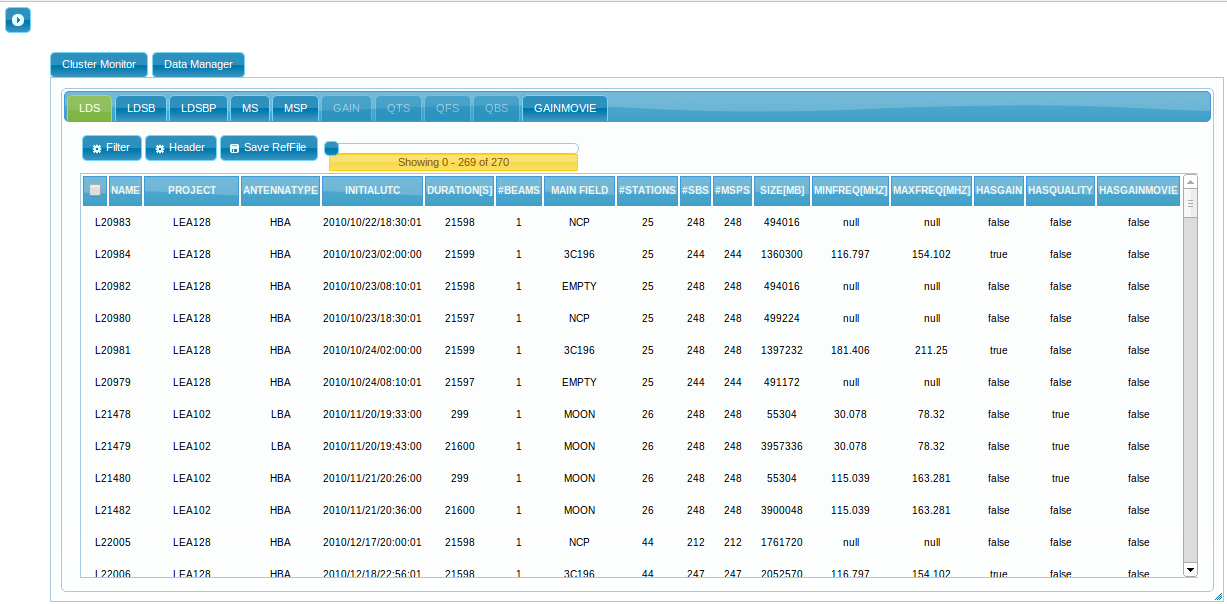
\includegraphics[scale=0.45]{fig/initwebui} 
	\caption{Snapshot of the LEDDB web UI}
	\label{fig:initwebui}
\end{figure}

\subsection{Query Engine}

The query engine is a python API which provides fast and flexible access to the database.

From the petabytes of data generated from the hundred of observations we estimate 10 terabytes of diagnostic data will be stored in the LEDDB (currently it is around 700 gigabytes). In addition to the size challenge, the number of rows of some of the tables is the most important issue to be taking into account for the design of the database and its query engine and it is actually the main bottleneck in the queries. We have managed to provide a fast access thanks to the table indexing, the minimization of the amount of join operations, the use of persistent connections eased by the session handling provided by the cherrypy framework and the direct query to the diagnostic partitions when possible.

The query engine provides functionality to sort, filter by column values and by selection in primary and secondary tables. In addition the queried columns can be changed. All this is used by the UI to provide a very extensive set of options for accessing the data.

The UI allows the user to create both \textit{RefFiles} and \textit{DiagFiles}. In addition to the database access, this UI can be used to launch pipeline jobs with a \textit{RefFile} and directly plot diagnostic data with a \textit{DiagFile} thanks to the \textit{DataManager} (see section \ref{sec:datamanager} for complete description on the \textit{DataManager}). \textit{ClusterMonitor} allows the user to see a snapshot of the current usage of the LOFAR EoR cluster nodes (see section \ref{sec:cm} for complete description on the \textit{ClusterMonitor}).

\subsubsection{Type of Queries}

There are ten type of queries (ten tabs in the LEDDB web UI). They are the ten primary tables described in section~\ref{sec:ref} and section~\ref{sec:diag}. 
Note that for LDS, LDSB, LDSBP and MS, each of this table is intrinsically joined with its related meta-data table.\\

If you want to change the type of query you just need to click on the corresponding tab. 
In all the query types you will see the following (apart from the \textit{DataManager} and \textit{ClusterMonitor} buttons which we will address in section \ref{sec:datamanager} and \ref{sec:cm}):

\begin{itemize}
	\item Show selected button: In the left top corner of the screen you can see a small button with a triangle icon. Once you make a selection, you can click this button to see a string with the selected elements comma-separated.
	
	\item Filter button: Click on this button to open the filtering window. More in section~\ref{sec:filtering}.
	
	\item Header button: Click on this button to open the header window. At any time you can change the columns that are displayed for each one of the main tabs.
	
	\item Other buttons depending on the tab: \textit{Save RefFile}, \textit{Save DiagFile}, \textit{Show Play Command} or \textit{Plot}.

	\begin{itemize}
		\item \textit{Save RefFile} button in the tabs related to referencing tables, i.e. LDS, LDSB, LDSBP, MS and MSP. More in section~\ref{sec:createref}.
		\item \textit{Save DiagFile} button in the tabs related to diagnostic tables, i.e. GAIN, QBS, QFS and QTS. More in section~\ref{sec:creatediag}.
		\item \textit{Show Play Command} button in the GAINMOVIE tab. When selecting a movie and clicking this button you will see a message box indicating the command that you should execute (in any node of the EoR cluster) in order to play the movie.
		\item \textit{Plot} button in the diagnostic tables. When selecting some diagnostic rows and clicking this button you will be redirected to a plotting UI (within the DataManager UI) that will allow you to do the plot online.
	\end{itemize}

	\item Sliding bar: Here you can see the total number of rows returned by the query. A maximum of 2000 rows are shown in each page. You can slide through the returned rows with the slider bar.
	
	\item Header: In the first row you see the column names. The first column is used to select/deselect all the rows. Pass the mouse though a column name and you will see a description of the column. You can click on it and the query will be re-executed sorting the results by the selected column. Click it again and the sorting will be inverted. You can at anytime modify the shown columns using the \textit{Header} button.
	
	\item Data rows: The rows returned by the LEDDB are shown here (only the first 2000 if more than 2000 rows are returned). You can select rows by clicking on them. Multiple-line selection is also possible.
\end{itemize}

In the Referencing tabs (LDS, LDSB, LDSBP, MS and MSP) any selection done in them will affect the queries of the tabs in the positions right of the current one. So, for example if you are in the LDS tab and you select one row, and then you go to the LDSB tab, only LDSBs related to the selected LDS will be shown. \\

The Diagnostic tabs GAIN, QBS, QFS and QTS are only activated if the previous tab was MS or LDSBP. There is a limit of 50 selected MSs or LDSBPs when querying for diagnostic data. This is done to avoid too expensive queries. The tab GAINMOVIE is always activated and can be used as any of the Referencing tabs.

\subsubsection{Filtering}
\label{sec:filtering}

When you click on a tab, by default all the rows of the related table are shown. As stated above, if you did any selection in a previous tab (in the left of the current one) only data related to the selected rows will be shown in the initial query of the new tab. You can also restrict the results by adding filters. To do so, click on the \textit{Filter} button and a new window will open similar to the one shown in figure \ref{fig:filterexample}. In the filter window there are two parts: Secondary-table filtering and column filtering. 

\begin{figure}[h]
	\centering
	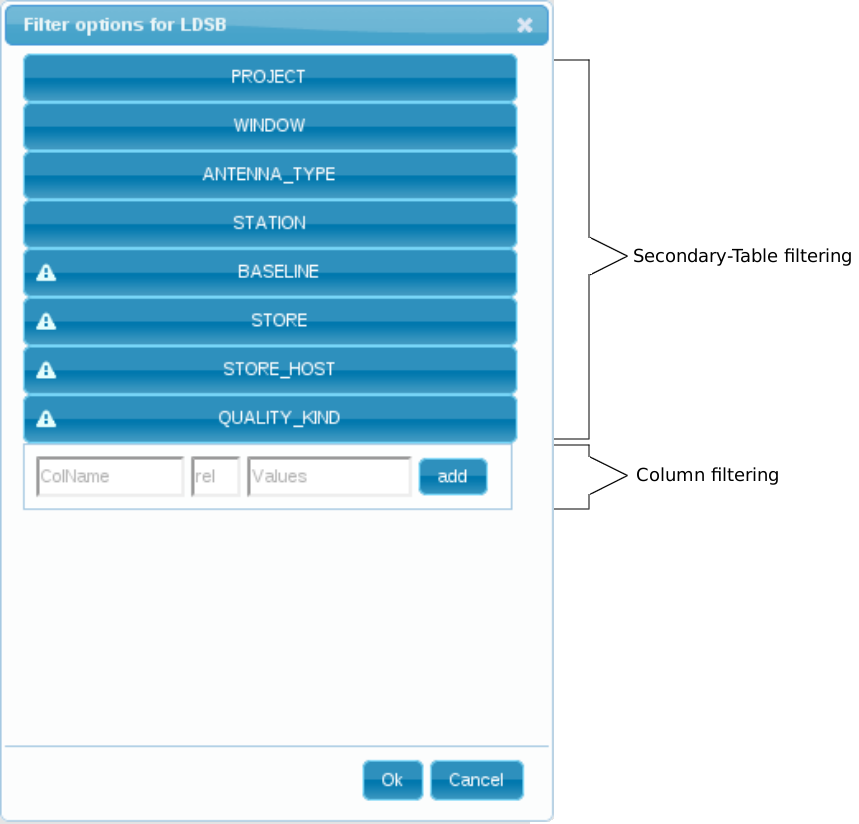
\includegraphics[scale=0.30]{fig/filterexample} 
	\caption{Filter window shown in the case of LDSB.}
	\label{fig:filterexample}
\end{figure}

\paragraph{Secondary-table filtering} 
In this part of the filter window you see the name of some of the secondary LEDDB tables. Those tables will help you to restrict what you select in the primary tables. This secondary tables can be in 3 states depending on the tab you are using:
\begin{itemize}
	\item enabled-active: Secondary tables in this state are enabled and they are related to the current tab, so any selection in these secondary tables will affect the current results. In the example in figure \ref{fig:filterexample} the secondary tables PROJECT, FIELD, ANTENNA\_TYPE and STATION are in enabled-active state.

	\item enabled-inactive: Secondary tables in this state (they are represented with an exclamation mark in a triangle) are enabled but they are not related to the current tab, so if you change them they will not affect the current results. However, they may affect future tabs (i.e. in the positions right of the current one) and may actually speed up the queries considerably. In the example in figure \ref{fig:filterexample} the secondary tables BASELINE, STORE, STORE\_HOST and QUALITY\_KIND are in enabled-inactive state. For example, if you are going to query some QBS, since queries to this table are very expensive, a very good way to speed them up is to previously select the QUALITY\_KIND in which you are interested. This will speed up the initial query done to QBS.

	\item disabled: Secondary tables in this state (represented by a shadowed blue) are disabled so you can not change them. This means you are in a tab where changing this secondary table will not affect current tab or future tabs (in the right of the current one). In the example in figure \ref{fig:filterexample} there is not any disabled secondary table.
\end{itemize}

It must be noted that when you add a secondary-table filter (i.e. make a selection in a secondary table) it will still be there in all the rest of tabs where it is enabled. 

If you click in any of the enabled ones, the related secondary table will be shown. You can select some rows and click on \textit{Ok} button to execute the new query with the filter you just added. You can also click on \textit{Back} to save the filter and go back to the filter menu to add other filters. 

Once you are in a secondary table selection you will see a text describing the type of logical decision the filter will do with your selection. In general, for all the secondary tables it is a logical \textit{OR}, which means that the returned rows will be related to at least one of the selected rows in the secondary table. The exception is \textit{STATION} in LDS, LDSB and LDSBP where it is an \textit{AND}.

\paragraph{Column filtering}
You can also add filters affecting the queried columns. If you click on the input box with the text \textit{ColName} you will see the possible columns names to which you can add a filter (these obviously depends on the tab you are). Once you select the column name click in the input box \textit{rel} to define the relation. The possible values are: \textit{=}, \textit{!=}, $>$, $<$, $\sim$ and $!\sim$. Finally if you click on the last white box you can define the values, several comments on this:

\begin{itemize}
	\item Booleans, strings (single-word), integers and floats are accepted.

	\item If the column is a boolean you can write: \textit{TRUE}, \textit{FALSE}, \textit{True}, \textit{False}, \textit{t}, \textit{f}, \textit{T} or \textit{F}.

	\item In the case of \textit{=} and \textit{!=} you can set multiple values. Use commas to separate them.

	\item In the case of \textit{=} and \textit{!=} in integer columns you can also use $..$ to make a range. For example $1..3$ is the same than $1,2,3$. Or $0..6..2$ is the same than $0,2,4,6$

	\item You can also query for \textit{null} (or not \textit{null}) columns using the \textit{=} and \textit{!=}.

	\item The operations $\sim$ and $!\sim$ are for string comparisons using POSIX regular expressions. For example to select all the fields which name is similar to NCP.
\end{itemize}
When you are done defining the values click on \textit{add} button (otherwise it will not be used). Then click on \textit{Ok} button and the query will be executed taking into account your filters.

Note that when you change the tab the columns filters will be reinitialized with the columns of the new tab. This is contrary to secondary-table filtering, so you can not add column filters that will affect other tabs.

\subsubsection{Query optimization}
\label{sec:queryengine}

There are many different ways to get the same data from the database. Some ways are faster than others. Here you have some tips about the query engine in order to optimize your queries:

\begin{itemize}
	\item Once you have a selection in a tab you can ``jump" tabs, i.e. for example you can select a LDS and directly go to MSP tab, then you will see all the MSPs related to the selected LDS. 

	\item Once you go to a tab when some selection was done in some other tabs in the positions left of it, the most restricting one will be used. For example, if you did a selection on LDS, then went to the LDSB and did another selection and finally you went to MSP, only the selection in LDSB will be used.

	\item If you select all the elements of a tab and then you change to a new tab, instead of using the selected values the query engine will use the same query parameters used in the previous tab. This is done to avoid expensive queries with unnecessary comparisons.

	\item When you select all the rows of a tab with more than one page it will be assumed you wanted to select all the rows of all the pages.

	\item And last but not least, we strongly recommend the usage of filters when possible, specially following these guidelines:
	\begin{itemize}
		\item Minimize the number of rows to select using filters (the fewer rows you select, the fewer comparisons the query engine must do).
		
		\item Try to use filters in order to make selection of all rows. Remember that when you select all the rows, the engine will implicitly use the filters you previously used to generate the next query.
		
		\item Use enable-inactive secondary-table filters (the ones that will affect tabs in the right of the current one). This will speed up the initial queries done when changing tab.
	\end{itemize}
	
	For example, if you want to query the GAIN solutions of the first forty sub-bands of an observation, let's define these three different approaches:
	\begin{itemize}
		\item Approach 1: Make a selection in LDSBP. Go to MS, select the first 40 rows. Go to GAIN.
	
		\item Approach 2: Make a selection in LDSBP. Go to MS and add a filter to see only sub-band indexes lower than 40. Select all the 40 MSs. Go to GAIN.
		
		\item Approach 3: Make a selection in LDSBP. Go to GAIN and add a filter to see only sub-band indexes lower than 40.
	\end{itemize}
	
	Of the three approaches the most optimal is the number 2. It this case there is only a single query to GAIN tab, and to generate the results there are only two comparisons for each GAIN row (one for the LDSBP and the other to check the sub-band index is lower than 40).  While in the first approach there will be 40 comparisons for each GAIN row (the 40 selected MSs). In third approach there are also only 2 comparisons but we have to query twice to GAIN tab and querying to the diagnostic tabs is always expensive.
	
	Now consider you want only core stations. The best way to do it would be to add the filter for core stations in LDSBP or MS tab. Even if it does not affect them when you add it, it would affect the results when you change to GAIN tab.
\end{itemize}


\subsection{Save RefFile}
\label{sec:createref}
It is possible to create a \textit{RefFile} from any of the tabs related to Referencing, i.e. LDS, LDSB, LDSBP, MS and MSP. Once you have done a selection, click on \textit{Save RefFile} button, a window will ask you for a name for the file. Once you click on \textit{Save} a new query will be done (to MSP table) to find all the measurement sets related to your selection. A temporary copy of the \textit{RefFile} will be stored in the LOFAR EoR cluster and the location will be shown. The user is responsible to copy this file to his home directory because every night these temporary files are deleted.

\subsection{Save DiagFile}
\label{sec:creatediag}
To be able to see any diagnostic data you must start from MS or LDSBP tabs and select less than 50 rows. Then you can go to one of the diagnostic tabs, i.e. GAIN, QBS, QFS and QTS. You can filter as in any other tab. Make a selection and click on \textit{Save DiagFile}. As in the case of the \textit{RefFile} this will ask you for the file name and will make a temporal copy of the file in the LOFAR EoR cluster.


\section{\textit{DataManager}}
\label{sec:datamanager}

The \textit{DataManager} web UI can be accessed from the main LEDDB web page by clicking the \textit{DataManager} button. If you do so, you will see a screen like the one in figure \ref{fig:dmwebui}.

\begin{figure}[h]
	\centering
	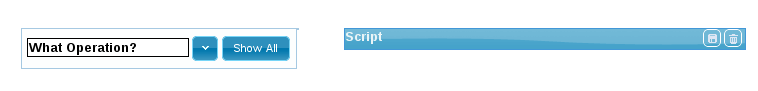
\includegraphics[scale=0.40]{fig/datamanagerinit} 
	\caption{Initial snapshot of the \textit{DataManager} web UI}
	\label{fig:dmwebui}
\end{figure}

If you already know the task you want, just type it in the input box. If you want to see all the available tasks click on \textit{Show All} button. To select a task, just click in its button. For example, in figure \ref{fig:copy} you see the UI window for the \textit{CopyData} task. Each task is a LModule (see LEDAMA document for more information regarding the LModules)

\begin{figure}[h]
	\centering
	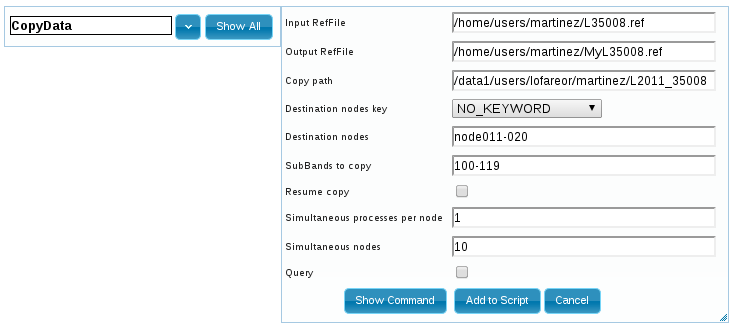
\includegraphics[scale=0.50]{fig/guicopy} 
	\caption{DataManager UI when \textit{CopyData} task is selected. You can also observe all the available tasks}
	\label{fig:copy}
\end{figure}

In all the tasks (or \textit{LModules}) you will see several running options (buttons):

\begin{itemize}
	\item \textit{Show Command}: Shows the command in a dialog box so you can copy it, paste it in a terminal and run it whenever and from wherever you want.
	
	\item \textit{Add to Script}: Adds the command (the same as shown in \textit{Show Command}) to a script. This is useful to design your own chain of tasks. The tasks you add to the script will be shown in the web UI. It must be noted that when you are done you must save the script (click on the Save button).
	
	\item \textit{Cancel}: Closes the current window. 
\end{itemize} 

\section{\textit{ClusterMonitor}}
\label{sec:cm}

Originally the table \textit{STORE\_HOST} in the LEDDB was also used to store the data required for the cluster monitor. Since it requires hundreds of update operations per second we decided to split this part from the LEDDB. Hence, there is another database which only contains the table \textit{STORE\_HOST} that is meant to fulfil this task. Currently this database is named NMDB and is running in node078.

From the LEDDB web UI we can also access to a Cluster Monitor web UI. With it, and using the previously stated database, we can see real-time information of the CPU, memory and NFS traffic of all the nodes of the LOFAR EoR cluster .

You can click on a node to see detailed information of it.

\pagebreak  

\section{Usage example}
\label{sec:usageexample}

This section describes a brief example of the usage of the LEDDB web UI and some example of usage for Data management and processing and diagnostic data analysis.

\subsection{LEDDB web UI}

Example use case: You want to find the last observation of NCP of 2011. Then, you want to create a \textit{RefFile} with the data in the LOFAR EoR cluster related to that observation. Finally, you want to see if there is any diagnostic data related to that observation and save some of it in a \textit{DiagFile}. 

In the querying, the proposed way is not the only one (in section \ref{sec:queryengine} you can find how to optimize your queries). You may find other ways to get the same results. This is just an example.

\begin{itemize}
	\item Step 1: Go to the LEDDB web and log in with the your LOFAR EoR cluster user and password.
	
	\item Step 2: By default the tab LDS is shown. Let's filter the LDSs, click on \textit{Filter} button to open the filters dialog. In the column filtering area, i.e. in the bottom, click on \textit{ColName} box and select \textit{mainField}, in the \textit{rel} box click on $\sim$ and in the \textit{values} box enter NCP. Click on \textit{add}.
	
	\item Step 3: Still on \textit{Filter} you are going to add a filter to see only data older than 2012. Again in the bottom, click on \textit{ColName} box and select \textit{initialUTC}, in the \textit{rel} box click on $<$ and in the \textit{values} box enter 2012/. Click on \textit{add} and then \textit{Ok}.
	
	\item Step 4: Now if you want to sort the rows by time, click on \textit{INITIALUTC} twice (this will sort them by time in descending order). The first row is the one you want. In this example, it is the observation \textit{L35008}, select it. Note that it has some quality data (column \textit{HASQUALITY} is \textit{True}).
	
	\item Step 5: This is a single-beam observation so LDSB contains only one row, you can go directly to the LDSBP tab. Here you will see two LDSBPs. One for data in LTA and the other for data in LOFAR EoR cluster. Let's filter the LTA data out. Click on \textit{Filter}. Now in \textit{STORE}, deselect all and select only EoR. Click on \textit{Ok}. Select the only row you see.
	
	\item Step 6: Click on \textit{Save RefFile}. If there is not any data in the EoR cluster you will see an error message. If there is data this will create a \textit{RefFile} with 244 MSPs (see \#MSPS column). Specify a file name, for example \textit{L35008.ref} and click on \textit{Save}. Copy the \textit{RefFile} to your home directory. You will need this \textit{RefFile} later.
	
	\item Step 7: Let's query some diagnostic data. First you need to select some MSs or LDSBPs. In this case we will use the already selected LDSBP. In order to ease the QTS query we will already add the \textit{QUALITY\_KIND} filter. In this example we are interested in the \textit{Count} (number of unflagged samples). Click on \textit{Filter}, click on \textit{QUALITY\_KIND}, deselect all and select only \textit{Count}. Click \textit{Ok}. This will not change the shown LDSBPs because the filter you just added does not apply yet but you will need to select the LDSBP again.
	
	\item Step 8: Click on QFS tab. Thanks to the previously added filter, we will only see data where \textit{QUALITY\_KIND} is \textit{Count}.
	
	\item Step 9: Select all the rows. 
	
	\item Step 9: Click in \textit{Save DiagFile}. This will also create a temporary file in the cluster. Copy it to your home directory. 
	
	\item Step 10 (alternative): In this point, after selecting all the rows, another option would be to click on \textit{Plot QFS} button. If you press this button a temporal \textit{DiagFile} will be automatically created and you will be redirected to the \textit{DataManager} \textit{QTSPlotter} window where the input \textit{DiagFile} will be automatically filled up.
\end{itemize}

At this point you have already created a \textit{RefFile} and a \textit{DiagFile}. Let's do something with them in the following sections.

\subsection{Data Management and Processing}

Example use case: You want to make a copy of measurement sets in a \textit{RefFile}. Then, you want to run NDPPP to make a average version of those measurement sets. We will assume that we could create the \textit{RefFile} in the previous section. However, this example would be the same for any \textit{RefFile} referencing all the MSPs of an observation stored in the EoR cluster. 

\begin{itemize}
	\item Step 1: Use a terminal to go to some node of the LOFAR EoR cluster.

	\item Step 2: Let's test how to make a copy of the data. Let's see the two options you have for this step: 

	\begin{itemize}
		\item The first option is to use the command-line tool \textit{ExecuteLModule} (see LEDAMA document for more information). The command is:
			\begin{verbatim}
ExecuteLModule CopyData -i /home/users/martinez/L35008.ref
-o /home/users/martinez/MyL35008.ref -c /data1/users/martinez/L2011_35008
-u node011-020 -b 100-119 -p 1 -n 10
			\end{verbatim}
			In the command-line tool you can use \textit{ExecuteLModule CopyData -h} to see all the possible arguments.
		\item The second option is to use the \textit{DataManager} web UI (click on \textit{DataManager} in the main LEDDB web UI page). 
			\begin{itemize}
				\item Click on \textit{Show All} button.
	
				\item Click on \textit{CopyData} button.
	
				\item Type in the path to the input RefFile. 
	
				\item Fill the rest of input arguments as shown in figure \ref{fig:guicopy} (some of the arguments are automatically filled up). 
	
				\item Click on \textit{Show command}.
					\begin{figure}[h]
						\centering
						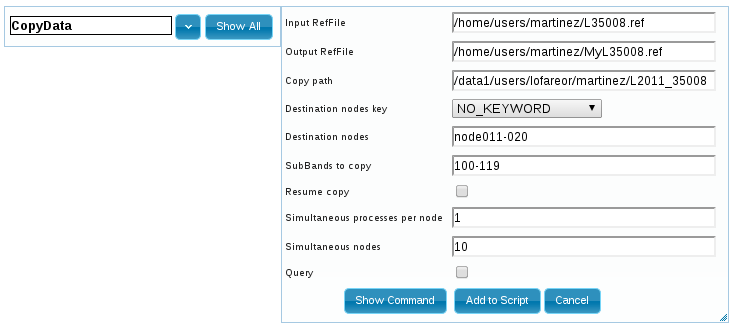
\includegraphics[scale=0.50]{fig/guicopy} 
						\caption{Copy window in \textit{DataManager} web UI with user-defined arguments}
						\label{fig:guicopy}
					\end{figure}
			\end{itemize} 
		\item Copy the command and paste it in a terminal (in any node of the LOFAR EoR culster).
	\end{itemize}

	Note that with both options you end up with the same command. This command will copy the sub-bands 100 to 119 to nodes node011 to node020, so each node will have two sub-bands (\textit{CopyData} will distribute the sub-bands in the selected nodes minimizing the difference between number of sub-bands in the different nodes in case of a total number of sub-bands not being multiple of number of nodes). The ten nodes will be receiving data simultaneously. Each node will have only one simultaneous copy process. In order to be able to make this copy the parent directory of the copy path (\textit{/data1/users/martinez} in the example) must be created in the destination nodes and you must have write permissions on it. Contact the system administrator for this purpose.

	From now on we will show the command to run the tasks. As in the CopyData case you can get it using the command-line launcher (\textit{ExecuteLModule}) or with the \textit{DataManager} web UI.

	\item Step 3: In order to run NDPPP you first need to create the parset files. We need to use the \textit{CreateNDPPPParsetFiles}. The command is:\begin{verbatim}
ExecuteLModule CreateNDPPPParsetFiles -i /home/users/martinez/MyL35008.ref 
-t /home/users/martinez/NDPPP/NDPPP_average.parset
-o /home/users/martinez/L35008_NDPPP_parsets 
-c /data1/users/martinez/L2011_35008_001 -p 1 -n 10
\end{verbatim}

This will create NDPPP parsets for the measurement sets in \\ \textit{/home/users/martinez/MyL35008.ref} and will place them in the folder \\  \textit{/home/users/martinez/L35008\_NDPPP\_parsets}. Each parset will be generated using as a template the one in \textit{/home/users/martinez/NDPPP/NDPPP\_average.parset} but changing \textit{msin} and \textit{msout}. In this case you will write the output measurement sets in the \textit{/data1/users/martinez/L2011\_35008\_001} (the nodes to use are defined when running NDPPP).

	\item Step 4: When you are done with generating the NDPPP parsets you can proceed to running NDPPP. For this you can use the \textit{LaunchNDPPP}. The command is:
\begin{verbatim}
ExecuteLModule LaunchNDPPP -i /home/users/martinez/L35008_NDPPP_parsets 
-l /home/users/martinez/L35008_NDPPP_logs
-p 1 -n 10
\end{verbatim}
Note that the nodes are not specified. If no nodes are specified the nodes containing the original data are used. The logs of the several NDPPP executions will be written to \\ \textit{/home/users/martinez/L35008\_NDPPP\_logs}. In addition to the log files you can also use the \textit{ClusterMonitor} to see the status of your tasks.

	\item Step 5: Once NDPPP is done, if you want to do more tasks with the recently created data you need to create a \textit{RefFile} of it. Since this data is not in the LEDDB (references to user data are not stored in the LEDDB) you need to use the \textit{CreateRefFileFromPath} for this purpose. The command is:
\begin{verbatim}
ExecuteLModule CreateRefFileFromPath -i /data1/users/martinez/L2011_35008_001
-s node011-020 -o /home/users/martinez/MyL35008_001.ref -p 1 -n 10
\end{verbatim}
	
\end{itemize}

Another option to do all these steps all together is via the \textit{Script} option in the \textit{DataManager} web UI. See section \ref{sec:datamanager} for more information on \textit{Script}.

\subsection{Diagnostic Data Analysis}

Example use case: You want to use the \textit{DiagFile} to get a plot of the number of unflagged samples of all the sub-bands of L35008 as a function of frequency.

We will plot the diagnostic data via the Data Manager web UI. Whether you clicked on Plot QFS or you created a DiagFile and then went to DataManager you end up in the same place. Fill the parameters as in figure \ref{fig:plotqfs}

\begin{figure}[h]
	\centering
	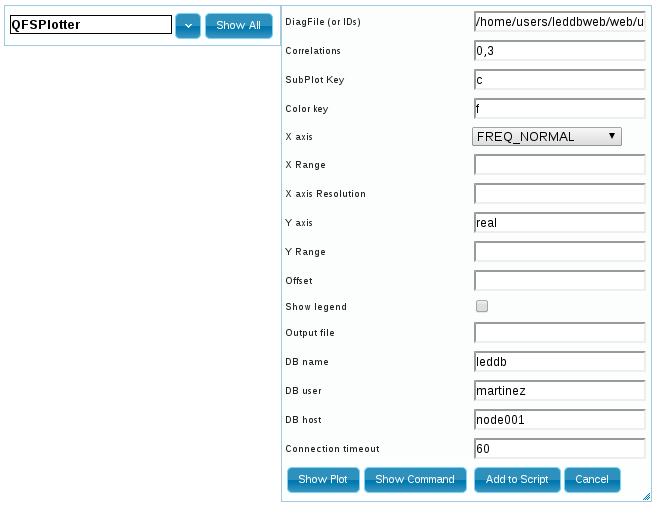
\includegraphics[scale=0.5]{fig/plotqfs} 
	\caption{Parameters required to get the plot. Note that we only plot XX and YY, set the x axis to frequency, define a subplot for each correlation, different color for each subband and only plot real complex coordinate (since in this case imaginary part is always 0)}
	\label{fig:plotqfs}
\end{figure}

Another option would be to use the command-line plotter (see LEDAMA document for more information). The command would be is:
\begin{verbatim}
ExecuteLModule QFSPlotter -i L35008_QTS.diag -g 0,3 -s c -c f -x FREQ_NORMAL -y real
\end{verbatim}

Independently of what you use to get the plot, it must be the same than figure \ref{fig:l35008qfs}.

\begin{figure}[h]
	\centering
	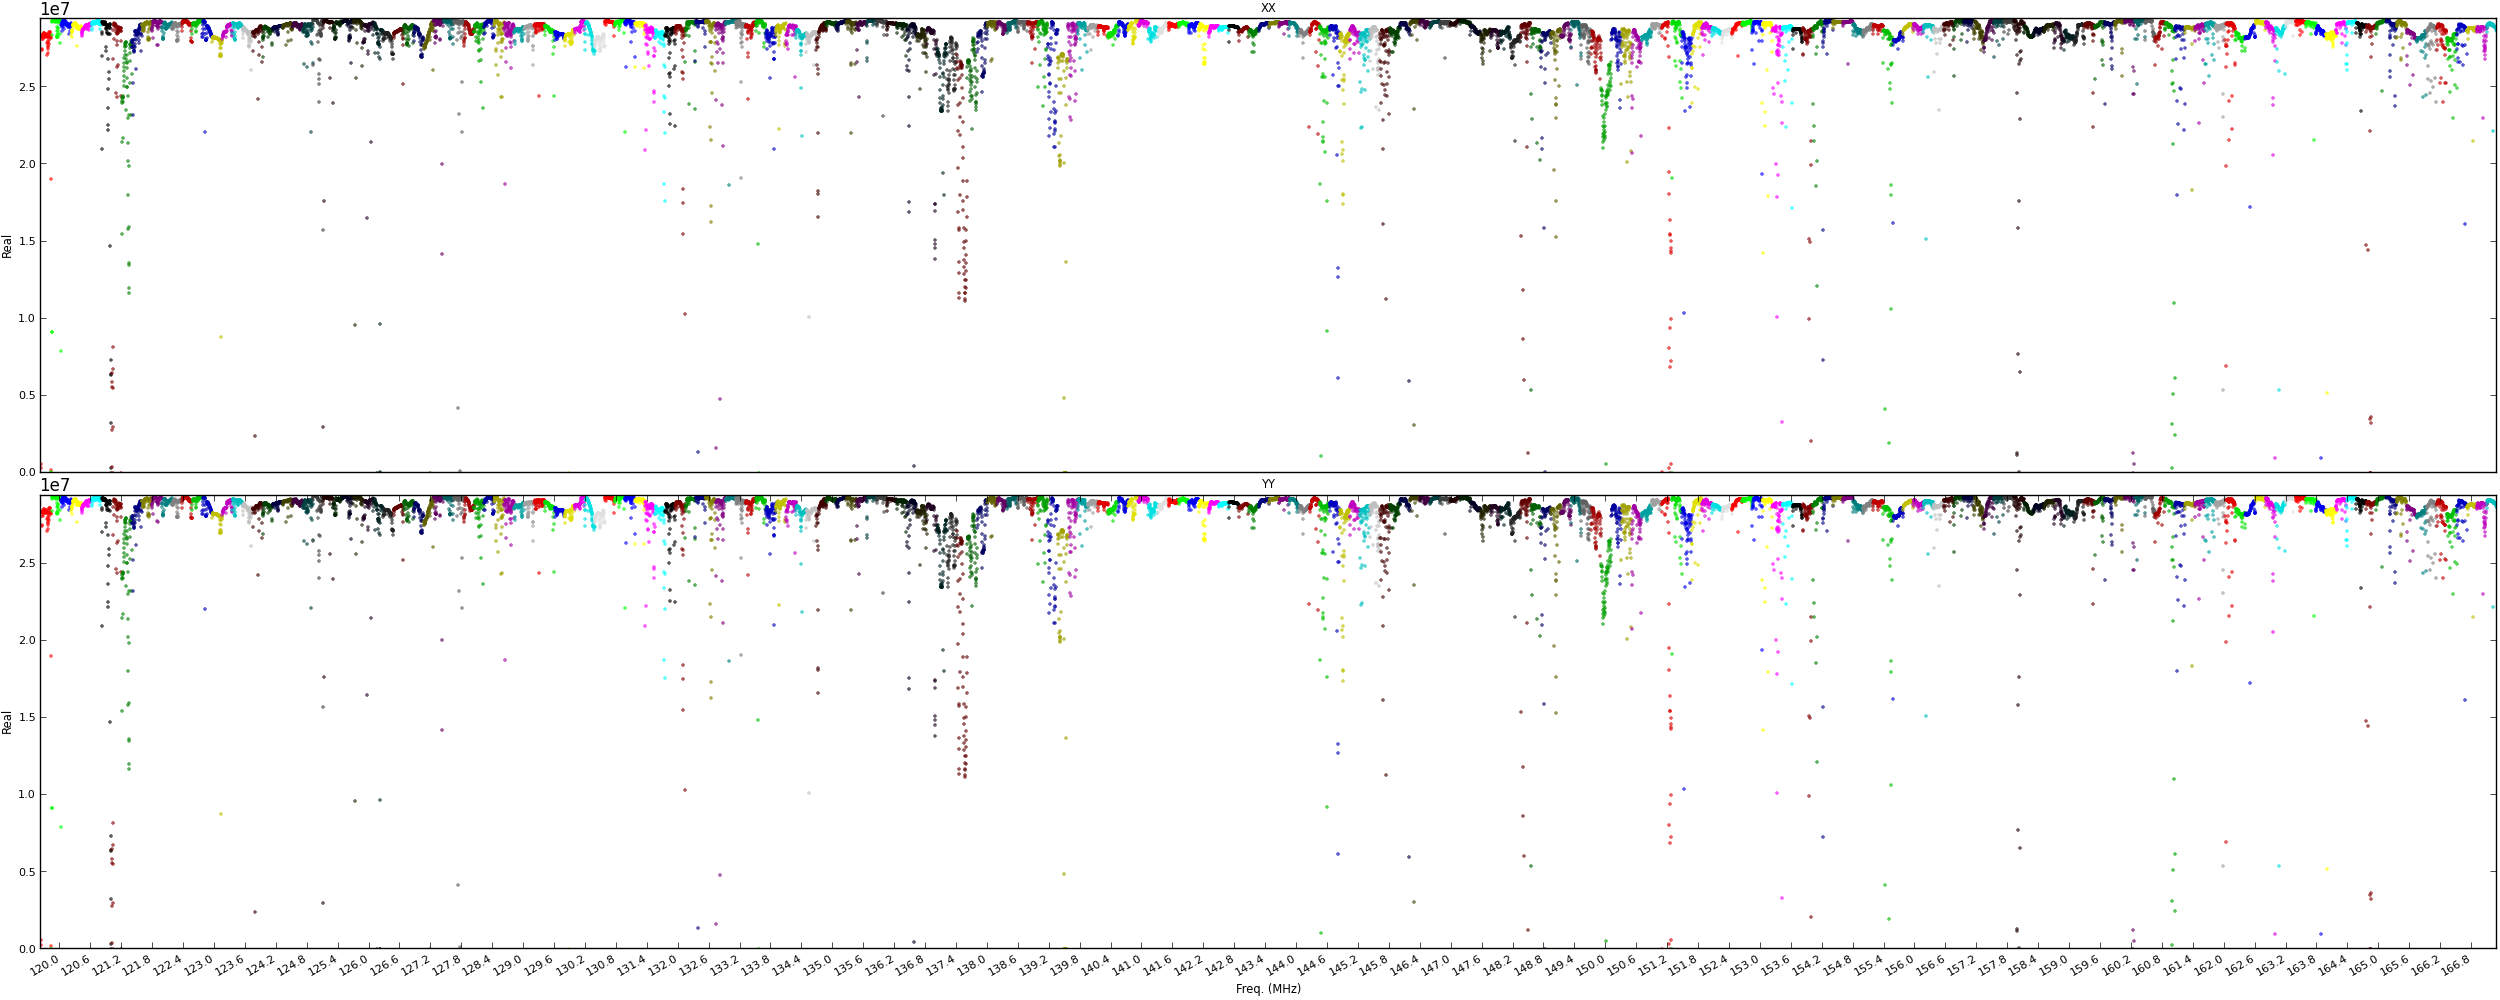
\includegraphics[scale=0.25]{fig/l35008qfs} 
	\caption{Number of unflagged samples in all the sub-bands of L35008 as a function of frequency. Each point is the number of unflagged samples for a frequency channel}
	\label{fig:l35008qfs}
\end{figure}

\subsubsection*{Acknowledgments}

None of the above could have been done without A. G. de Bruyn, S. Zaroubi, L. Koopmans, M. Brentjens, V. Veligatla, E.Tiesinga, V. Jelic, V.N. Pandey, S. Yatawatta, P. Lampropoulos, A. R. Offringa. Thank you.

\end{document}
